\documentclass{zbc-report}

%% Set up the bibliography
\usepackage{biblatex}
\addbibresource{report.bib}

%% Additional packages and commands
\usepackage{parskip}
\setlist{itemsep=-2pt} % Reducing white space in lists slightly
\renewcommand{\deg}{\si{\degree}\xspace} % Use \deg easily, everywhere

%% Set up the minted package
\usepackage[cachedir=_minted-report]{minted}
\setminted{
    linenos=true,
    breaklines=true,
    fontsize=\footnotesize,
    frame=lines,
    framesep=2mm,
    baselinestretch=1.2,
    bgcolor=gray!10,
    style=vs,
    mathescape=true,
}

%% ----------------------------------------------------------------------
%%    Begin of document + Frontmatter (Roman page numbering)
%% ----------------------------------------------------------------------

\begin{document}

\frontmatter

%% Define the main parameters
\title{Databaser}
\subtitle{Mandatory assignment \\ Software Design}
\author{Carsten Lydeking}

\subject{Computer Science} % Cover only
\large\affiliation{Zealand Business College} % Cover only
\coverimage{figures/binary} % Aspect ratio of 2:3 (portrait) recommended
\definecolor{title}{HTML}{4884d6} % Color for cover title

\makecover

\begin{titlepage}

\begin{center}

%% Print the title
{\makeatletter
\largetitlestyle\fontsize{45}{45}\selectfont\@title
\makeatother}

%% Print the subtitle
{\makeatletter
\ifdefvoid{\@subtitle}{}{\bigskip\titlestyle\fontsize{20}{20}\selectfont\@subtitle}
\makeatother}

\bigskip
\bigskip

%% Print the name of the author
{\makeatletter
\largetitlestyle\fontsize{25}{25}\selectfont\@author
\makeatother}

\bigskip
\bigskip

%% Print table with names and student numbers
\setlength\extrarowheight{2pt}
\begin{tabular}{c}
    cal002@edu.zealand.dk \\
\end{tabular}

\vfill

%% Print some more information at the bottom
\begin{tabular}{l r}
    Teacher:         & M. Lynggaard Krarup\\
    Report Deadline: & \ddmmyydate{03/05/24} \\
    Handed-in:       & \ddmmyydate{\today} \\
    Faculty:         & Computer Science \\
\end{tabular}

\bigskip
%% Add a source and description for the cover and optional attribution for the template
\begin{tabular}{l r}
    Cover: & Generated image of binary using DALL-E \\
    Style: & TU Delft Report Style -- modified by Carsten Lydeking \\
\end{tabular}


%% Insert the Zealand logo at the bottom of the page
\begin{tikzpicture}[remember picture]
    \node[above=10mm] at (current page.south) {%
        
\includegraphics[width=0.35\textwidth]{figures/zealandcombinedlogo}
    };
\end{tikzpicture}

\end{center}

\end{titlepage}

\tableofcontents
%\listoffigures
%\listoftables

\chapter*{Nomenclature}
\addcontentsline{toc}{chapter}{Nomenclature}

\section{Abbreviations and definitions}
\label{sec:abbreviations}
The following abbreviations and definitions are used throughout the report:

\renewcommand{\arraystretch}{2}
\begin{longtable}{l p{13.5cm}}
    \textbf{Abb.}  & \textbf{Definition}  \\ \hline
        DB           & Database: A structured collection of data stored electronically. \\ \hline
        RDB          & Relational Database: A type of DB that stores and provides access to data points that are related to one another. \\ \hline
        DBMS         & Database Management System: Software that handles the storage, retrieval, and updating of data in a database. \\ \hline
        RDBMS        & Relational DBMS: A database management system based on the relational model introduced by E.F. Codd. \\ \hline
        SQL          & Structured Query Language: A programming language used to manage and manipulate relational databases. \\ \hline
        CRUD         & Create, Read, Update, Delete The four basic operations of persistent storage: adding, retrieving, modifying, and removing data. \\ \hline
        GUI          & Graphical User Interface  A user interface that allows users to interact with electronic devices using graphical icons and visual indicators. \\ \hline
        PK           & Primary Key:A unique identifier for each record in a database table. \\ \hline
        FK           & Foreign Key: A field in a database table that links to the primary key of another table. \\ \hline
        NML          & Normalization: In relation to RDB design, the process of organizing the columns (attributes) and tables (relations) to minimize data redundancy. \\ \hline
        1NF          & First Normal Form: A stage of NML where each table has atomic (i.e. indivisible) values and each record needs to be unique. \\ \hline
        2NF          & Second Normal Form: A stage of NML where it meets all the requirements of the 1NF and does not have partial dependency. \\ \hline
        3NF          & Third Normal Form: A stage of NML where it meets all the requirements of the 2NF and has no transitive functional dependencies. \\ \hline
        ERD          & Entity Relationship Diagram: A graphical representation of entities and their relationships to each other, typically used in database design. \\ \hline
        UML          & Unified Modeling Language: A standardized modeling language used to specify, visualize, construct, and document the artifacts of software systems. \\ \hline
        DDL          & Data Definition Language: A subset of SQL used to define database structures, such as tables, schemas, and databases. \\ \hline
        DML          & Data Manipulation Language: A subset of SQL used for adding (inserting), deleting, and modifying (updating) data in a database. \\ \hline
        DCL          & Data Control Language: A subset of SQL used to control access to data in a database. \\ \hline
        TCL          & Transaction Control Language: A subset of SQL used to manage the changes made by DML statements. \\ \hline
        XML          & Extensible Markup Language: A markup language that defines a set of rules for encoding documents in a format that is both human-readable and machine-readable. \\ \hline
        JSON         & JavaScript Object Notation: A lightweight data-interchange format that is easy for humans to read and write, and for machines to parse and generate. \\ \hline
    \renewcommand{\arraystretch}{1}
\end{longtable}

%% ----------------------------------------------------------------------
%%    Mainmatter (Arabic page numbering)
%% ----------------------------------------------------------------------

\mainmatter

\chapter{Introduction}
\label{chapter:introduction}

\section{The Report}
This report is written in \LaTeX  in VS Code with the \LaTeX  Workshop extension.
A template has also been prepared for use by other students at Zealand. It is expected that this will be made available on GitHub at a later date.
As a strong opposer of \emph{Danglish}, I have chosen to write in english, as it is the base language for the applied software scripts, programming languages and terminology.

\section{Used Tools}
\begin{itemize}
    \item \LaTeX  - For writing the report
    \item Visual Studio Code v. 1.60.2 - With \LaTeX  Workshop extension for editing
    \item Visual Studio 2022 Enterprise Edition v. 17.8.0 - For application development
    \item GitHub - For version control
    \item Microsoft SQL Server Management Studio v. 19.3 - For database development
    \item Microsoft SQL Server 2022 - For hosting the database
\end{itemize}

\section{Purpose}
This report has been prepared as part of the curriculum for Software Design at Zealand. The report deals with a case where a database is to be developed for a fictitious company. In addition, an application is to be developed that can access the database.
Furthermore an application is to be developed that can access the database.

\section{The assigmnet}
Has been copied verbatim from Moodle and is as follows:

\subsection{Afleveringsformat}
Følgende uploades i WiseFlow:
\begin{itemize}
    \item En rapport på PDF format
    \item En reference til jeres kode uploades sammen med rapporten enten som ZIP-fil eller med en reference til GitHub i rapporten.
\end{itemize}

\subsection{Opgaven:}
\begin{enumerate}
    \item Lav en database model (Hint: beskriv attributes, relationer, multiplicitet, primary keys (PK) og foreign keys (FK)).
    \item Redegør for, at dine tabeller er på 3je Normalform.
    \item Lav et SQL script over, hvorledes du kan oprette de nødvendige tabeller.
    \item Lav din database, så den indeholder tabellerne.
    \item Indsæt nogle passende værdier.
    \item Lav en Windows Form Applikation (eller console applikation), så den kan lave CRUD på faciliteter.
\end{enumerate}

Besvarelsen skal indeholde de nødvendige oplysninger, så jeres lærer kan afprøve jeres applikation.

\chapter{The database}
\label{chapter:the-database}

\section{Database Model}
The logic behind the database is to keep track of reservations, customers, hotels, rooms and facilities.
The database is designed to handle reservations of rooms at hotels, and to keep track of customer information and what facilities the hotels offer.

This results in the database consisting of the following tables:
\begin{itemize}
  \item Hotels
  \item Customers
  \item Rooms
  \item Reservations
  \item Facilities
  \item HotelFacilities
\end{itemize}

\subsection{Relations and Multiplicity}

\begin{itemize}
  \item A Hotel can have many Rooms (1 to Many)
  \item A Customer can have many Reservations (1 to Many)
  \item A Room can be part of one Reservation at a time (1 to Many)
  \item Facilities are shared among Hotels through HotelFacilities (Many to Many)
\end{itemize}

\subsection{3NF State}
All tables are in 3NF because:
\begin{enumerate}
  \item They are in 1NF as all attributes are \emph{atomic} - no groups are repeated or contain more than one value.
      This can be seen, for example, by HotelFacilities being a relationship table between Hotel and Facility.
  \item They are in 2NF as there is no \emph{partial dependency} - Non-key columns depend solely on the PK.
      This can be seen, for example, by Hotel having a relationship to Facility instead of containing Facility as an attribute.
  \item There are no \emph{transitive dependencies} - Non-key columns depend only on the PK.
      This can be seen, for example, by Room having a relationship to Hotel instead of containing Hotel as an attribute.
\end{enumerate}

\section*{Diagrams}
The diagrams should be simple enough to be self-explanatory. The DMD is created first and based on the many-to-many relationship between hotels and facilities, it gives rise to an index table (HotelFacilities).
In the DMD, HotelFacilities is not considered as an independent entity but rather as a way to manage the relationship between Hotel and Facilities.

\begin{figure}
  \centering
  \begin{subfigure}[b]{0.45\textwidth}
    \centering
    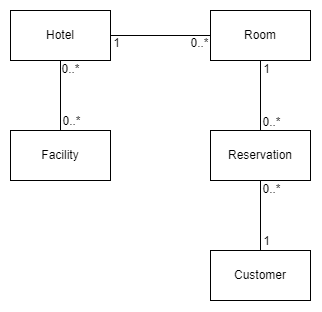
\includegraphics[width=\textwidth]{figures/SWD_Domain_HotelManagement.png}
    \caption{Domain Model Diagram}\label{DomainModelDiagram}
  \end{subfigure}
  \hfill
  \begin{subfigure}[b]{0.45\textwidth}
    \centering
    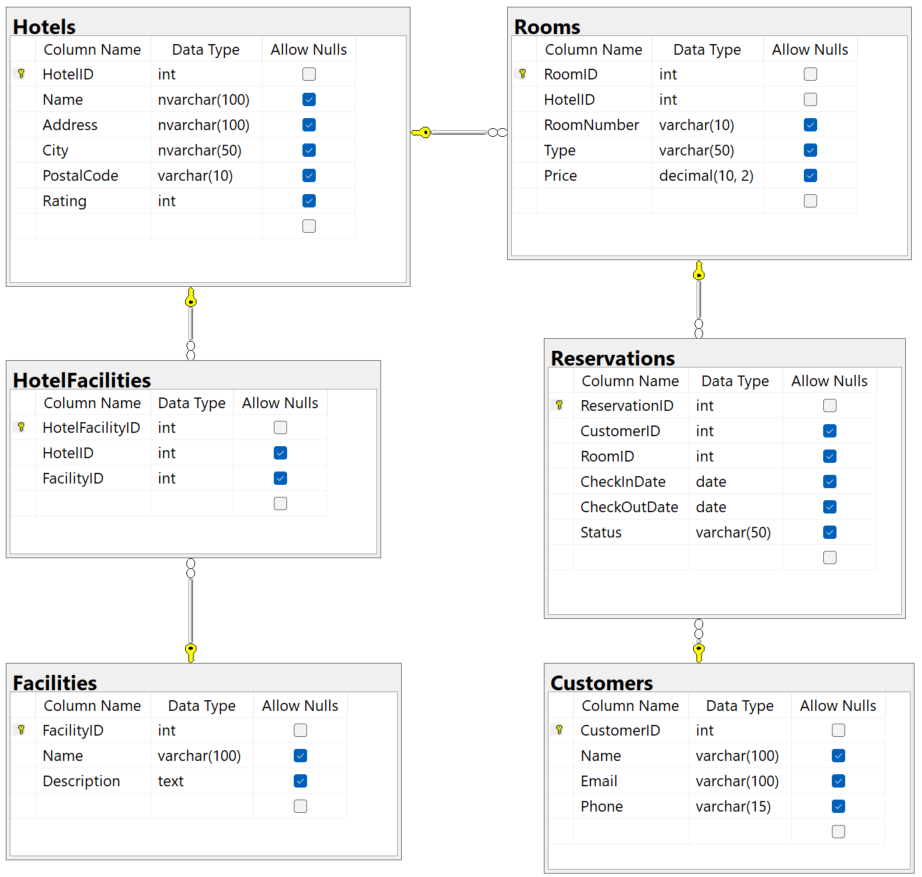
\includegraphics[width=\textwidth]{figures/SWD_ERD_HotelManagement.png}
    \caption{Entity Relationship Diagram}\label{EntityRelationDiagram}
  \end{subfigure}
  \caption{Domain Model and Entity Relationship Diagrams}
\end{figure}

\subsection{Domain Model Diagram}
See Figure 1. This DMD only contains entities, multiplicities, and relationships.
This provides input on how the database should be designed based on the individual tables and their relationships to each other.

\subsection{Entity-Relationship Diagram}
See Figure 1. The ERD is generated from the tables in the database and shows the relationships between the tables, their PK, FK, and data types.

\chapter{Database Diagrams}
\label{chapter:diagrams}

\section{Models and relationships}
The diagrams should be simple enough to be self-explanatory. The DMD is created first and based on the many-to-many relationship between hotels and facilities, it gives rise to an index table (HotelFacilities).
In the DMD, HotelFacilities is not considered as an independent entity but rather as a way to manage the relationship between Hotel and Facilities.
The ERD is then created from the DMD and shows the relationships between the tables, their PK, FK, and data types.

\subsection{Domain Model Diagram}
See figure \ref*{fig:domain-model-diagram}. 
This DMD only contains entities, multiplicities, and relationships.
This provides input on how the database should be designed based on the individual tables and their relationships to each other.

\begin{figure}
  \centering
  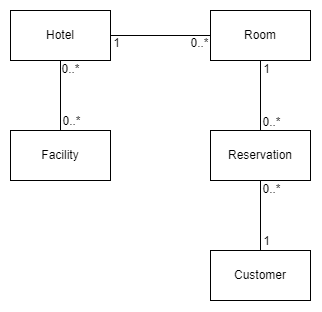
\includegraphics[width=0.75\textwidth]{figures/SWD_Domain_HotelManagement.png}
  \caption{Domain Model Diagram}
  \label{fig:domain-model-diagram}
\end{figure}

\pagebreak

\subsection{Entity-Relationship Diagram}
See figure \ref*{fig:entity-relationship-diagram}. 
The ERD is generated from the tables in the database and shows the relationships between the tables, their PK, FK, and data types.

\begin{figure}
  \centering
  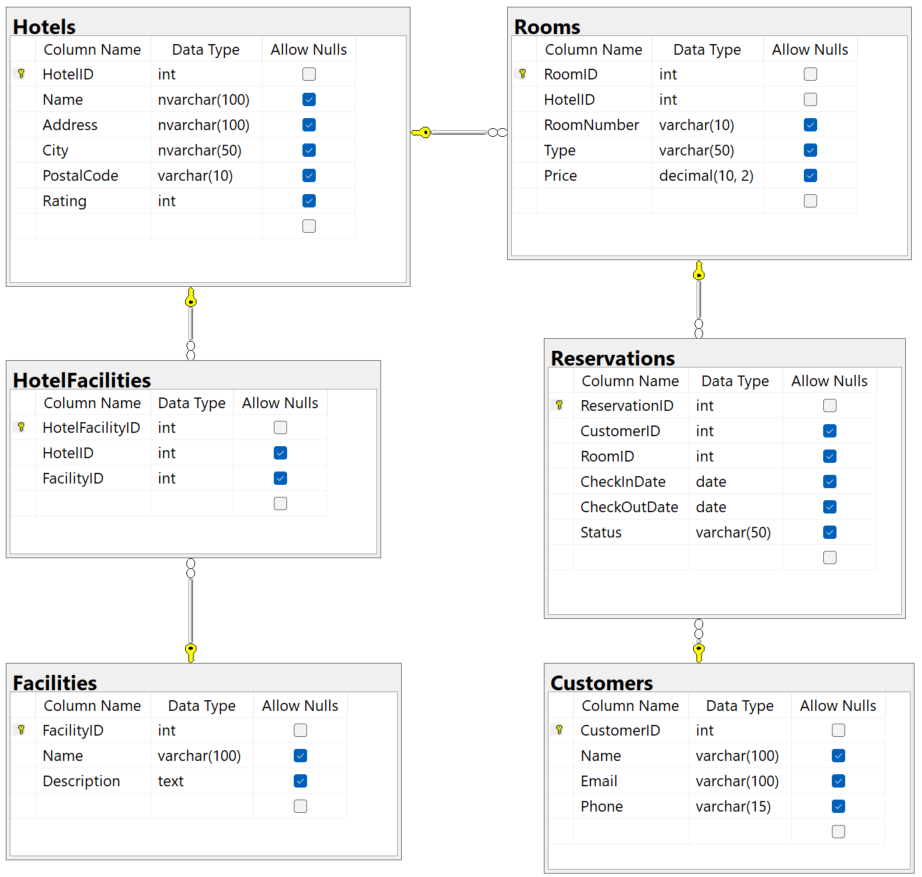
\includegraphics[width=0.75\textwidth]{figures/SWD_ERD_HotelManagement.png}
  \caption{Entity Relationship Diagram}
  \label{fig:entity-relationship-diagram}
\end{figure}

\chapter{Conclusion}
\label{chapter:conclusion}

The purpose of this assignment was to design a database for a hotel management systemm, with an application that could do CRUD operations on the Facilities table. 
While this has been an academic excersise, the focus has been on the process of designing and implementing a database, and not on the application (UI and UX) itself.

The report has details this process, diving into the thoughts behind designing the database, including the requirements, the design, and the implementation. 

Furthermore, the report entails the process of creating a database schema and the process of implementing the database schema in a SQL database. 
This was enhanced upon with a WinForms application that could interact with the database.

The database has been designed and implemented according to the requirements, and the application has been tested to ensure that it can perform the CRUD operations on the Facilities table.
Overall, the assignment will be regarded as a success, and the process has been a learning experience.

%% Prevent urls running into margins in bibliography
\setcounter{biburlnumpenalty}{7000}
\setcounter{biburllcpenalty}{7000}
\setcounter{biburlucpenalty}{7000}

%% Add bibliography
\printbibliography[heading=bibintoc,title={References}]

%% ----------------------------------------------------------------------
%%    Appendix (Letters for chapters)
%% ----------------------------------------------------------------------

\appendix

\chapter{SQL Schema}

\section{Tabels}
This section contains the SQL code for creating the tables in the database.

\begin{lstlisting}[language=SQL]{codefiles/CreateAllTables.sql}

\section{Mock Data}
This section contains the SQL code for inserting mock data into the tables.

\begin{lstlisting}[language=SQL]{codefiles/DanishMockData.sql}


\end{document}